\section{I2C fundamentals}
\label{chap:i2c}

As we will be leveraging the \gls{I2C} protocol, it is worth looking into the inner workings. 

\gls{I2C}~\cite{nxp:i2c} is a serial communication bus invented in the eighties by Philips Semiconductors. It uses only two bidirectional lines, a \gls{SDA} and a \gls{SCL}. Typically, 7-bit addressing is used, but there exists a 10-bit extension. This extension is fully backwards compatible, allowing a software-emulated 10-bit addressing implementation if the hardware only supports 7-bit addressing.

This communication bus has no minimum frequency, but can go as fast as 5 Mbit/s. Not every \gls{MCU} supports every frequency though, for example the PCF8523 Real-Time Clock only supports up to 1 MHz.

Besides a 0 or 1 data bit, there are two special START and STOP signals which act as message delimiters.

% [in principe kan er nog verteld worden over de verschillende snelheden en dergelijke, maar aangezien ik daar niet mee te maken heb gehad ben ik van mening dat dat hier out of scope is]
\subsection{Operations}

A node on the bus can have one of two roles\footnote{In earlier literature, the terminology master and slave were used for respectively controller and target.}:
\begin{itemize}
    \item Controller: Generates the clock, via required minimum periods for the low and high phases of the \gls{SCL}, and initiates communication with targets.
    \item Target: Receives the clock and responds when addressed by the controller.
\end{itemize}
Any number of any type can be present, and these may be changed between messages. They can also both receive and send data, when in the corresponding mode.

Initial communication is established by a controller that sends a START followed by the address of the target it wishes to communicate with, which is finally completed by a single bit indicating if it wishes to write (0) or read (1) from the target. If the target exists on the bus, it will respond with an acknowledgement. This \gls{ACK} corresponds with transmitting a single 0 bit, there is also a \gls{NACK} which is a single 1 bit.

\begin{figure}[h]
    \centering
    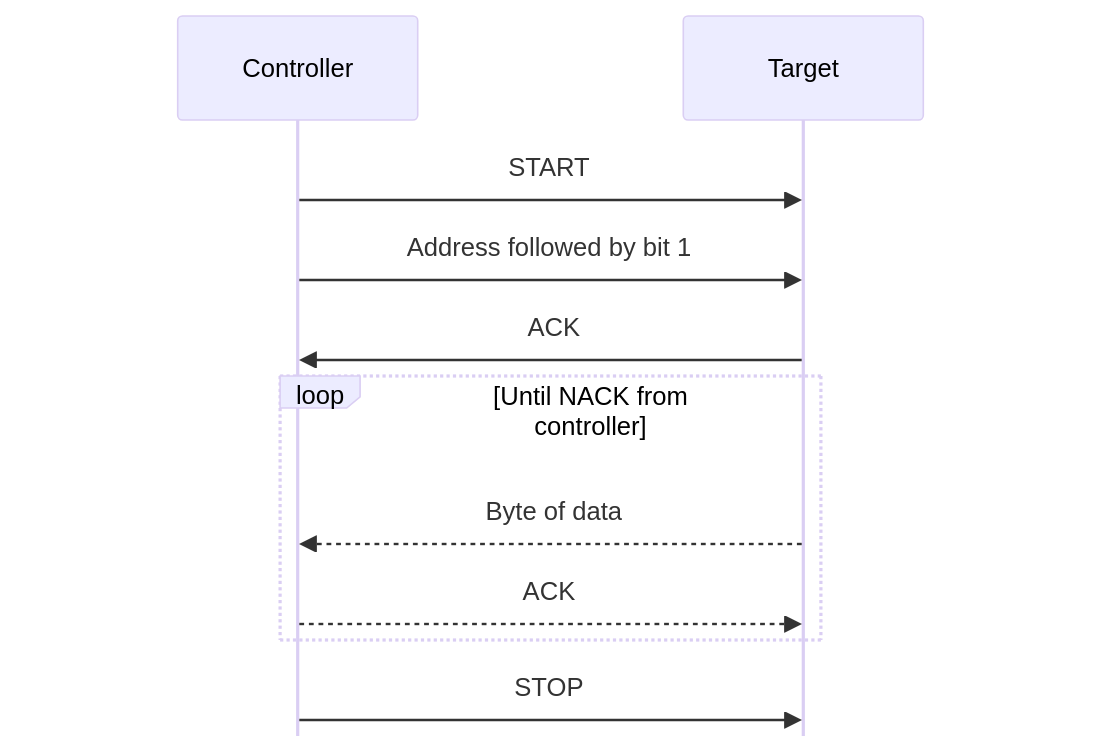
\includegraphics[width=0.5\textwidth]{figures/read_example.png}
    \caption{Example sequence of a read operation.}
    \label{fig:read_example}
\end{figure}

Further communication is performed by one party sending data, most significant bit first, and the other sending an \gls{ACK} bit.

\subsubsection{Bus sharing}

In the case of multiple targets linked with one controller, the controller needs to indicate which target it wants to interact with. To achieve this, each target compares the address sent by the controller with its own. If the address matches, it sends a low voltage \gls{ACK} bit back to the controller. If the address doesn't match, the target does nothing and the \gls{SDA} line remains high.

When there are multiple controllers, issues can arise, precisely when they try to send or receive data at the same time over the \gls{SDA} line. To solve this problem, each controller needs to detect if the \gls{SDA} line is low or high before transmitting a message. If the \gls{SDA} line is low, another controller is in control of the bus, and it should wait until a STOP has been received to send the message. If the \gls{SDA} line is high, then it's safe to transmit the message.

\subsubsection{Methods}

The protocol defines three basic types:
\begin{itemize}
    \item Write: Controller writes bytes to the target.
    \item Read: Controller reads bytes from the target until a given buffer is full.
    \item Write-read: Controller first writes bytes and then reads enough bytes to fill the buffer in a single transaction.
\end{itemize}

It is also possible to combine a list of write and read operations inside a transaction contract.
Figure \ref{fig:read_example} showcases more in detail how a read operation works.

\subsection{SMBus}
% [het idee is dat er hier uitgelegd gaat worden van wat SMBus is en de relatie met I2C]

The \gls{SMBus}~\cite{smbus} is a subset derived from \gls{I2C} by Intel. Its main application is to monitor critical parameters on PC motherboards and in embedded systems. On the surface they are quite similar, but there are some subtle differences worth mentioning. For one, \gls{SMBus} will time out when \gls{SCL} is held low for more than 35 milliseconds. \gls{I2C} doesn't have an established timeout value, implicating that a target or controller can hold \gls{SCL} as long as necessary to process data. \\
On account of this timeout, \gls{SMBus} has a minimum clock speed of 10 kHz. Leading to a maximum of 100 kHz. As stated earlier, \gls{I2C} can go as fast as 5 Mbit/s and no minimum frequency is specified.

Another difference is in terms of voltage levels. For \gls{I2C} the typical levels are +5 V, +3.3 V or even +1.8 V and below. In contrast, in an \gls{SMBus} system the supply ranges are restricted between +1.8 V and +5 V. In general, even with the different specifications for the input logic voltage thresholds, \gls{I2C} and \gls{SMBus} devices will be interoperable over the supply voltages permitted by the SMBus specification.

Sometimes libraries that provide methods for \gls{I2C} communication, also provide ones for \gls{SMBus}. But, thus, in the context of driving an \gls{I2C} target device, these can be safely ignored.

